\newpage

\appendix

\section*{\LARGE Appendix}

\section{Model Intelligence Index}
\label{sec:appendix-intelligence-index}

To quantify the capabilities of LLMs used in our study, \textcolor{black}{we adopt while extending the \textit{Artificial Analysis Intelligence Index} (\url{https://artificialanalysis.ai/evaluations/artificial-analysis-intelligence-index}).} This index provides a publicly available synthesis of model capabilities, combining performance across reasoning, knowledge, mathematics, coding, instruction following, long-context reasoning, and agentic workflow tasks. Its construction integrates eight evaluation suites (e.g., MMLU-Pro \citep{wang2024mmlu}, GPQA Diamond \citep{rein2024gpqa}, HLE \citep{phan2025humanity}, AIME 2025, SciCode \citep{tian2024scicode}, LiveCodeBench \citep{jain2025livecodebench}, IFBench \citep{pyatkin2025generalizing}, AA-LCR \citep{artificialanalysis2025lcr}, Terminal-Bench Hard, and $\tau^2$-Bench Telecom \citep{barres2025t2bench}), with careful standardization, robust answer extraction, and model-agnostic prompting. 

Our study requires a unified, quantitative measure of a model’s baseline capabilities that is \emph{independent of} any agentic mechanism or multi-agent collaboration structure. The Intelligence Index meets this requirement by:  
(i) evaluating all models under consistent, zero-shot, instruction-prompted conditions;  
(ii) employing pass@1 scoring and robust equality-checker mechanisms;  
(iii) reporting a composite measure reflecting general-purpose reasoning and problem-solving ability; and  
(iv) demonstrating high statistical reliability (reported confidence interval below $\pm 1\%$).  
This makes it suitable as a foundational axis for studying \textit{how agentic performance scales with underlying model capacity}.

\paragraph{Beyond Artificial Analysis Evaluations.}  
Artificial Analysis reports Intelligence Index scores for a growing but still limited subset of frontier models. Our work requires a broader coverage, including several models that are not yet benchmarked on the official platform. For these models, we independently reproduced a subset of the Intelligence Index evaluations, specifically AA-LCR \citep{artificialanalysis2025lcr}, HLE \citep{phan2025humanity}, MMLU-Pro \citep{wang2024mmlu}, GPQA Diamond \citep{rein2024gpqa}, AIME 2025, LiveCodeBench \citep{jain2025livecodebench}, SciCode \citep{tian2024scicode}, and IFBench \citep{pyatkin2025generalizing} using the publicly disclosed methodology, prompts, scoring procedures, and evaluation environments described by Artificial Analysis. 

For the models without publicly available results, we computed a \textit{reconstructed Intelligence Index} following the equal-weighting formulation used in Intelligence Index v3.0. In cases where full reproduction was infeasible (e.g., specific agentic workflow tasks or unavailable context window limits), we report approximate estimates (denoted with *) and discuss their limitations transparently. These reconstructed values should be interpreted as \emph{methodologically consistent but not officially certified} estimates.


Table~\ref{tab:intelligence_index} summarizes the reconstructed Intelligence Index and underlying component scores for all models used in our study. The table includes:  
(i) official Intelligence Index values when available;  
(ii) reconstructed values for non-reported models;  
(iii) all constituent evaluation scores used to compute the aggregate index;  
(iv) additional model metadata (context window, cost, throughput, latency) relevant for agentic performance analysis.



\begin{table*}[ht!]
\centering
\caption{Intelligence Index (non-agentic capability) for LLMs used in our experiments.}
\label{tab:intelligence_index}
\resizebox{\textwidth}{!}{
\begin{tabular}{lccccccccc}
\toprule
Model & \textbf{Index} & AA-LCR & HLE & MMLU-Pro & GPQA Diamond & AIME 25 & LiveCode & SciCode & IFBench \\
\midrule
\raisebox{-0.1\height}{
\includegraphics[height=1em]{imgs/openai-logo.png}} GPT-5.2 & 75 & 73 & 31 & 87 & 90 & 99 & 89 & 52 & 75 \\
\raisebox{-0.1\height}{
\includegraphics[height=1em]{imgs/openai-logo.png}} GPT-5              & 71 & 76 & 27 & 87 & 85 & 94 & 85 & 43 & 73 \\
\raisebox{-0.1\height}{
\includegraphics[height=1em]{imgs/openai-logo.png}} GPT-5 mini         & 68 & 68 & 20 & 84 & 91 & 84 & 84 & 39 & 75 \\
\raisebox{-0.1\height}{
\includegraphics[height=1em]{imgs/openai-logo.png}} GPT-5 nano         & 59 & 42 & 8 & 78 & 84 & 79 & 79 & 37 & 68 \\
\hdashline
\raisebox{-0.1\height}{
\includegraphics[height=1em]{imgs/gemini-logo.png}} Gemini-3.0 Pro     & 75 & 71 & 37 & 90 & 91 & 96 & 92 & 56 & 70 \\
\raisebox{-0.1\height}{
\includegraphics[height=1em]{imgs/gemini-logo.png}} Gemini-3.0 Flash   & 75 & 66 & 35 & 89 & 90 & 97 & 91 & 51 & 78 \\
\raisebox{-0.1\height}{
\includegraphics[height=1em]{imgs/gemini-logo.png}} Gemini-2.5 Pro     & 65 & 66 & 21 & 86 & 84 & 88 & 80 & 43 & 49 \\
\raisebox{-0.1\height}{
\includegraphics[height=1em]{imgs/gemini-logo.png}} Gemini-2.5 Flash   & 58 & 57 & 13 & 84 & 79 & 78 & 63 & 41 & 52 \\
\raisebox{-0.1\height}{
\includegraphics[height=1em]{imgs/gemini-logo.png}} Gemini-2.0 Flash   & 47 & 45$^*$ & 8$^*$ & 77 & 68$^*$ & 73 & 39$^*$ & 35$^*$ & 30$^*$ \\
\hdashline
\raisebox{-0.1\height}{
\includegraphics[height=1em]{imgs/claude-logo.png}} Claude Sonnet 4.5  & 55 & 66 & 7 & 88 & 83 & 37 & 71 & 43 & 43 \\
\raisebox{-0.1\height}{
\includegraphics[height=1em]{imgs/claude-logo.png}} Claude Sonnet 4  & 47 & 62$^*$ & 5$^*$ & 87 & 75 & 21 & 56$^*$ & 38$^*$ & 35$^*$ \\
\raisebox{-0.1\height}{
\includegraphics[height=1em]{imgs/claude-logo.png}} Claude 3.7 Sonnet & 42 & 58$^*$ & 2$^*$ & 81 & 67 & 12 & 57 & 32$^*$ & 30$^*$ \\
\bottomrule
\end{tabular}
}
\vspace{1mm}
\raggedright
\footnotesize{$^*$ Estimated or averaged from reported range.}
\end{table*}


Our reconstructed Intelligence Index values should be interpreted with appropriate caution.  
First, several evaluations, particularly long-context and agentic workflow tasks, contain nondeterministic components that may vary slightly across implementations.
Second, for models without public API support for large-context evaluation (e.g., ``non-reasoning'' checkpoints), our long-context estimates represent upper-bound approximations based on available context windows and internal model behavior.  
Third, Artificial Analysis maintains private test variants and additional filtering procedures that cannot be fully reproduced. Thus, our estimates provide a methodologically aligned but not officially verified extension.


\begin{table}[t]
\caption{Aggregate out-of-sample validation metrics across three held-out models (GPT-5.2, Gemini-3.0 Pro, Gemini-3.0 Flash) on BrowseComp-Plus, all with Intelligence Index = 75. The scaling equation achieves well-calibrated MAS predictions while systematically over-predicting single-agent performance.}
\label{tab:validation_summary}
\centering
\begin{tabular}{l c c}
\toprule
\textbf{Metric} & \textbf{Value} & \textbf{Note} \\
\midrule
Overall MAE & 0.077 & 15 predictions \\
MAS-only MAE & 0.061 & 12 predictions \\
SAS-only MAE & 0.138 & 3 predictions \\
\midrule
Overall MAPE & 19.9\% & --- \\
MAS-only MAPE & 15.3\% & --- \\
\midrule
Findings Validated & 11/15 & 73\% \\
Findings Partial & 2/15 & 13\% \\
\bottomrule
\end{tabular}
\end{table}

\begin{table*}[t]
\caption{Architecture-wise prediction accuracy for three held-out models on BrowseComp-Plus. All models share Intelligence Index = 75. MAS predictions are well-calibrated (average error 6.1\%), while SAS shows systematic over-prediction due to linear extrapolation beyond the training range.}
\label{tab:architecture_predictions}
\footnotesize
\centering
\begin{tabular}{l ccc ccc ccc}
\toprule
& \multicolumn{3}{c}{\textbf{GPT-5.2}} & \multicolumn{3}{c}{\textbf{Gemini-3.0 Pro}} & \multicolumn{3}{c}{\textbf{Gemini-3.0 Flash}} \\
\cmidrule(lr){2-4} \cmidrule(lr){5-7} \cmidrule(lr){8-10}
\textbf{Architecture} & Pred. & Actual & Error & Pred. & Actual & Error & Pred. & Actual & Error \\
\midrule
SAS & 0.521 & 0.450 & $+$15.8\% & 0.521 & 0.360 & $+$44.7\% & 0.521 & 0.340 & $+$53.2\% \\
MAS-Centralized & 0.480 & 0.480 & $+$0.0\% & 0.480 & 0.440 & $+$9.1\% & 0.480 & 0.480 & $+$0.0\% \\
MAS-Decentralized & 0.496 & 0.480 & $+$3.3\% & 0.496 & 0.500 & $-$0.8\% & 0.496 & 0.400 & $+$24.0\% \\
MAS-Independent & 0.413 & 0.350 & $+$18.0\% & 0.413 & 0.400 & $+$3.2\% & 0.413 & 0.360 & $+$14.7\% \\
MAS-Hybrid & 0.560 & 0.390 & $+$43.6\% & 0.560 & 0.440 & $+$27.3\% & 0.560 & 0.400 & $+$40.0\% \\
\midrule
\textbf{MAE (Overall)} & \multicolumn{3}{c}{0.064} & \multicolumn{3}{c}{0.068} & \multicolumn{3}{c}{0.098} \\
\textbf{MAE (MAS only)} & \multicolumn{3}{c}{0.062} & \multicolumn{3}{c}{0.044} & \multicolumn{3}{c}{0.077} \\
\bottomrule
\end{tabular}
\end{table*}


\begin{table*}[t]
\caption{Validation of key findings from Section~\ref{sec:results} across three held-out models. Three findings generalize universally (\textcolor{green!60!black}{\ding{51}}), while two show model-family-specific patterns. Per-model validation rates are 4/5, 4/5, and 3/5 respectively.}
\label{tab:findings_validation}
\footnotesize
\centering
\begin{tabularx}{\textwidth}{X c c c}
\toprule
\textbf{Finding} & \textbf{GPT-5.2} & \textbf{Gemini-3.0 Pro} & \textbf{Gemini-3.0 Flash} \\
\midrule
Capability Ceiling (higher $P_{SA}$ correlates with diminishing MAS returns) 
& \textcolor{green!60!black}{\ding{51}} & \textcolor{green!60!black}{\ding{51}} & \textcolor{green!60!black}{\ding{51}} \\

Independent MAS Degradation (Independent underperforms SAS)
& \textcolor{green!60!black}{\ding{51}} & \textcolor{red!60!black}{\ding{55}}$^\dagger$ & Partial$^\dagger$ \\

Optimal Architecture (Centralized/Decentralized excel)
& \textcolor{green!60!black}{\ding{51}} & \textcolor{green!60!black}{\ding{51}} & \textcolor{green!60!black}{\ding{51}} \\

Hybrid Overhead (515\% overhead limits performance)
& \textcolor{green!60!black}{\ding{51}} & \textcolor{green!60!black}{\ding{51}} & \textcolor{green!60!black}{\ding{51}} \\

BrowseComp-Plus Pattern (Decentralized $\geq$ Centralized)
& Partial$^\ddagger$ & \textcolor{green!60!black}{\ding{51}} & \textcolor{red!60!black}{\ding{55}}$^\S$ \\
\midrule
\textbf{Total Validated} & \textbf{4/5} & \textbf{4/5} & \textbf{3/5} \\
\bottomrule
\end{tabularx}
\vspace{-4pt}
\begin{flushleft}
\footnotesize{$^\dagger$ Gemini models show Independent MAS matching or outperforming SAS (+11.1\% for Pro, +5.9\% for Flash), contrary to GPT-5.2 ($-$22.2\%). This may reflect model-family-specific agentic capabilities.} \\
\footnotesize{$^\ddagger$ GPT-5.2 shows convergence (both 0.48); main results predicted Decentralized advantage.} \\
\footnotesize{$^\S$ Gemini-3.0 Flash shows reversed pattern: Centralized (0.48) $>$ Decentralized (0.40).}
\end{flushleft}
\end{table*}


\begin{table}[t]
\caption{Model family differences despite identical Intelligence Index (75). Single-agent performance varies substantially across vendors, while best MAS performance converges, suggesting multi-agent architectures may compensate for single-agent limitations.}
\label{tab:model_family_differences}
\centering
\begin{tabular}{l c c c}
\toprule
\textbf{Model} & $P_{\text{SA}}$ & Best MAS & MAS Gain \\
\midrule
GPT-5.2 & 0.45 & 0.48 & $+$6.7\% \\
Gemini-3.0 Pro & 0.36 & 0.50 & $+$38.9\% \\
Gemini-3.0 Flash & 0.34 & 0.48 & $+$41.2\% \\
\bottomrule
\end{tabular}
\vspace{2pt}
\begin{flushleft}
\footnotesize{Note: All models share Intelligence Index = 75, yet exhibit different single-agent performance. This suggests Intelligence Index may not be directly comparable across model families.}
\end{flushleft}
\end{table}


\section{Out-of-Sample Validation}
\label{sec:validation}

To assess the generalizability of our scaling equation beyond the training distribution, we evaluate on three held-out models: GPT-5.2, Gemini-3.0 Pro, and Gemini-3.0 Flash. All three models share Intelligence Index = 75, representing extrapolation beyond our training range (Index 42--71) by approximately 5.6\%. Table~\ref{tab:validation_summary} summarizes aggregate validation metrics. Across 15 architecture-model combinations, the scaling equation achieves MAE = 0.077. MAS predictions are better calibrated (MAE = 0.061) than SAS predictions (MAE = 0.138), consistent with systematic over-prediction of single-agent performance when extrapolating beyond the training range.

\paragraph{Qualitative Findings Validation.}
Table~\ref{tab:findings_validation} evaluates whether the five key findings from Section~\ref{sec:results} generalize to held-out models. Across three models, 11 of 15 finding-model pairs validate (73\%), with two additional partial validations. Three findings generalize universally: (1) the capability ceiling effect persists across all models, (2) Centralized or Decentralized architectures achieve optimal performance, and (3) Hybrid overhead limits relative performance. Two findings show model-family-specific behavior: Independent MAS degradation validates only for GPT-5.2 but not for Gemini models, and the BrowseComp pattern (Decentralized $>$ Centralized) varies across model families.

\paragraph{Model Family Differences.}
An informative comparison arises from models with identical Intelligence Index (Table~\ref{tab:model_family_differences}). Despite Index = 75, single-agent performance varies substantially: GPT-5.2 achieves $P_{\text{SA}} = 0.45$, while Gemini-3.0 Pro and Gemini-3.0 Flash achieve 0.36 and 0.34, respectively. However, best MAS performance converges ($0.48$--$0.50$), suggesting that multi-agent architectures may compensate for single-agent limitations. Consequently, MAS gains are substantially higher for Gemini models (+38.9\% and +41.2\%) compared to GPT-5.2 (+6.7\%). This implies that Intelligence Index, while predictive within model families, may not be directly comparable across vendors, a limitation for cross-family extrapolation that future scaling laws should address.

\textbf{Architecture Selection Accuracy.} The scaling equation predicts Hybrid as optimal for all three models
($\hat{P}_{\text{Hybrid}} = 0.560$), yet empirically Centralized and Decentralized architectures achieve superior performance. This
discrepancy reflects two factors: (1) linear extrapolation of the intelligence effect ($\hat{\beta}_I = 0.126$) beyond its training
range, and (2) the model's failure to capture Hybrid's disproportionate overhead penalty at high capability levels. 
The equation systematically over-predicts Hybrid performance (mean error $+37.0\%$) while achieving reasonable calibration for Centralized (mean error $+3.0\%$) and Decentralized (signed mean error $+8.8\%$). These results suggest that while the scaling equation provides well-calibrated predictions for moderate-overhead architectures, high-overhead configurations like Hybrid require architecture-specific corrections when extrapolating to frontier models.


\section{Domain Complexity}
\label{appendix:domain_complexity}

\textcolor{black}{We characterize domain complexity through an ordinal score $D \in [0,1]$ that captures the degree of sequential interdependence and empirical difficulty across evaluated benchmarks. This characterization enables systematic analysis of when multi-agent coordination yields performance benefits versus incurring prohibitive overhead.}

\subsection{Complexity Score Assignment}

\textcolor{black}{Domain complexity $D \in [0, 1]$ is assigned based on three empirical task properties, each normalized to $[0,1]$:}

\begin{itemize}

    \item \textcolor{black}{\textbf{Sequential Interdependence.} The degree to which task completion requires strictly ordered reasoning steps. Tasks with parallelizable subtask structure (e.g., Finance Agent) score low, while tasks requiring sequential constraint satisfaction (e.g., PlanCraft) score high.}

    \item \textcolor{black}{\textbf{State-Space Complexity.} The extent of dynamic state evolution during task execution. Tasks with static or slowly evolving states score low, while tasks requiring tracking of rapidly changing environments (e.g., BrowseComp-Plus) score high.}

    \item \textcolor{black}{\textbf{Coordination Overhead Sensitivity.} Empirically observed degradation under multi-agent coordination relative to single-agent baselines, reflecting how much the task's structure penalizes inter-agent communication overhead.}
\end{itemize}

\textcolor{black}{The final score reflects the overall empirical difficulty profile, calibrated against observed MAS performance patterns across all configurations.}

\subsection{Domain Characterisation}

Table~\ref{tab:domain_complexity} summarises the complexity scores and defining characteristics of each benchmark.

\begin{table*}[h]
\centering
\caption{Domain complexity scores and task characteristics.}
\label{tab:domain_complexity}
\begin{tabular}{lcp{11.3cm}}
\toprule
\textbf{Domain} & \textbf{$D$} & \textbf{Characteristics} \\
\midrule
Workbench & 0.000 & Minimal sequential constraints; well-structured procedural reasoning with clear subtask boundaries; low coordination requirements \\
Finance Agent & 0.407 & Moderate decomposability; structured domains amenable to localised agent reasoning \\
PlanCraft & 0.419 & High sequential dependencies; constraint satisfaction requiring ordered reasoning steps \\
BrowseComp-Plus & 0.839 & Dynamic state evolution; complex visuospatial reasoning with interaction-heavy environments \\
\textcolor{black}{SWE-bench Verified} & \textcolor{black}{0.255} & \textcolor{black}{Decomposable software engineering tasks; multi-step codebase exploration with test feedback; high tool count (7)} \\
\textcolor{black}{Terminal-Bench} & \textcolor{black}{0.414} & \textcolor{black}{Diverse CLI tasks with varying difficulty; Docker-based environments; low tool count (2)} \\
\bottomrule
\end{tabular}
\end{table*}

\subsection{Critical Threshold}

Our analysis identifies a critical complexity threshold at $D \approx 0.40$. Below this threshold, multi-agent architectures yield net positive returns through effective task decomposition and parallel reasoning. Above this threshold, coordination overhead consumes computational resources otherwise allocated to reasoning, resulting in performance degradation. This finding suggests that the suitability of multi-agent approaches is fundamentally constrained by domain-intrinsic properties rather than architectural sophistication alone.


\section{Datasets}

\textcolor{black}{We evaluate our agent systems across six agentic benchmarks requiring multi-step reasoning and tool interaction. Each dataset emphasizes different aspects of agentic behavior: information retrieval, domain expertise, planning, task decomposition, software engineering, and terminal-based task execution.}

\paragraph{Finance Agent.}

We use the Finance Agent benchmark \citep{bigeard2025finance}, comprising 50 finance questions requiring domain expertise and multi-step analysis. Tasks include earnings analysis, financial metric calculations, and market trend interpretation. Each instance includes expert-provided rubrics for structured evaluation. Questions typically require 15-30 minutes of expert time, indicating substantial complexity. 

\paragraph{BrowseComp Plus.}
BrowseComp Plus \citep{chen2025browsecomp} contains 100 web browsing tasks requiring multi-website information synthesis. Tasks include comparative analysis, fact verification, and
multi-source research across the web. Each instance requires agents to navigate multiple websites, extract relevant details, and synthesize findings. The dataset uses LLM-based evaluation comparing agent responses against ground truth answers with confidence scoring.

\paragraph{WorkBench.}
WorkBench \citep{styles2024workbench} evaluates business task automation through function calling sequences. The dataset covers five domains: analytics, calendar management, email
operations, project management, and customer relationship management. Success requires executing correct tool sequences to accomplish realistic business workflows. Evaluation follows outcome-centric assessment, measuring exact match between predicted and expected function call sequences. The dataset supports 100 distinct business scenarios with tolerance for minor date variations.

\paragraph{Plancraft.}
Plancraft \citep{dagan2024plancraft} focuses on sequential planning in Minecraft environments. Agents must craft target items by determining optimal action sequences using available inventory and crafting recipes. Tasks require multi-step reasoning about dependencies, resource management, and action ordering. The dataset uses environment-determined success
metrics based on successful item crafting within step limits. We use the plancraft-test subset containing focused planning challenges.

\textcolor{black}{\paragraph{SWE-bench Verified.}
SWE-bench Verified \citep{jimenez2023swe} evaluates software engineering capabilities through real-world GitHub issue resolution. Each instance provides a repository snapshot and issue description; agents must produce a patch that resolves the issue and passes the repository's test suite. The benchmark provides 7 tools including bash execution, file editing, directory navigation, search, and test execution, requiring multi-step codebase exploration, hypothesis generation, and iterative debugging. We evaluate on a 20-instance subset selected via deterministic shuffle (seed 42) from the 500-instance verified split, balancing computational cost with coverage across repository diversity.}

\textcolor{black}{\paragraph{Terminal-Bench.}
Terminal-Bench \citep{merrill2026terminal} evaluates CLI task execution across diverse system administration, security, machine learning, and debugging scenarios. Each instance specifies a terminal task with a Docker-based evaluation environment and objective success criteria. Agents interact through 2 tools (bash command execution and answer submission), requiring sustained environmental interaction under varying time limits. We evaluate on the first 20 instances from the 86-instance benchmark, covering tasks ranging from file manipulation and network configuration to model training and system diagnostics.}

\section{Implementation Details}

\subsection{Technical Infrastructure}

\textcolor{black}{Our implementation uses LiteLLM (\url{https://www.litellm.ai/}) for unified API access across model providers and LangChain (\url{https://www.langchain.com/}) for agent orchestration and tool integration.} LiteLLM provides standardized interfaces for OpenAI, Gemini, and Anthropic models, enabling seamless model switching and comparison. LangChain facilitates tool binding, conversation management, and structured prompting.

\paragraph{API Integration.}

We access LLMs through provider-specific APIs: OpenAI API for GPT models (gpt-5, gpt-5-mini, gpt-5-nano), GenAI API for Gemini models (gemini-2.5-pro, gemini-2.5-flash, gemini-2.0-flash), and Anthropic API for Claude models (claude-4.5-sonnet, claude-4.0-sonnet, claude-3.7-sonnet). Our implementation includes intelligent API key rotation across multiple keys per provider to handle rate limiting and quota management. Context window management automatically truncates conversation history when token limits are approached.

\paragraph{Tool Environment.}
Each dataset defines its tool ecosystem through environment configurations. \textcolor{black}{Tools include web search (Tavily, \url{https://tavily.com/}), code execution} (Python REPL), mathematical operations, and task
completion markers. Tool definitions use LangChain's BaseTool interface with structured input schemas and execution methods. Tools are dynamically bound to LLM instances using
function calling capabilities when available.

\subsection{Agent Configuration}

\paragraph{Architecture Parameters.}
Single agents use maximum 10 iterations per instance. Independent multi-agent systems deploy 3 agents with synthesis-only coordination. Centralized systems employ 3 sub-agents with 1 orchestrator across maximum 5 orchestration rounds, with 3 iterations per agent per round. Decentralized systems run 3 agents through 3 debate rounds with 3 iterations per round. Hybrid systems combine centralized orchestration with limited peer communication phases.

\paragraph{Heterogeneous Models.}
Our framework supports heterogeneous configurations where different agent roles use different models. Orchestrators can use high-capability models (e.g., GPT-5) while sub-agents use
efficient models (e.g., Gemini-2.0 Flash). The LLMConfig class manages model assignment with automatic LLM instance creation for each agent role. Decentralized systems can assign
different models to different workers for diversity.

\subsection{Prompt Compilation System}

We implement a structured prompting system supporting named templates and variable interpolation. Prompts are defined in YAML files with base templates and role-specific extensions.
The compilation process performs template variable replacement using double-brace syntax ({{variable}}) and supports conditional template selection based on agent type and conversation state.

\paragraph{Dataset Integration.}
Each dataset provides shared prompt templates containing task-specific instructions and examples. Dataset instances contribute prompt variables including problem descriptions,
context, and constraints. The prompt compilation system merges agent prompts with dataset templates, ensuring consistent instruction delivery across architectures while maintaining task specificity.

\subsection{Evaluation Methodology}

\paragraph{Sample Sizes.}
\textcolor{black}{We evaluate on dataset subsets balancing computational cost with statistical significance: Finance Agent (50 instances), BrowseComp Plus (100 instances), WorkBench (100 instances), Plancraft (100 instances), SWE-bench Verified (20 instances, deterministic shuffle with seed 42 from 500), and Terminal-Bench (20 instances, first-$N$ from 86). The smaller subsets for SWE-bench Verified and Terminal-Bench reflect the computational cost of Docker-based evaluation environments; bootstrap 95\% confidence intervals are reported in Table \ref{tab:s6_bootstrap}.} Instance selection ensures representative coverage of task types and difficulty levels within each benchmark.

\paragraph{Restrictions and Controls.}
All experiments use identical tool interfaces and observation structures across architectures to eliminate external feedback confounds. Context window management applies consistent truncation policies. API rate limiting and retry mechanisms ensure fair resource allocation. Evaluation uses frozen model weights without fine-tuning to measure architectural effects independently of model optimization.

\subsection{Information Gain Computation}
\label{appendix:info_gain}

Information gain $\Delta\mathcal{I}$ quantifies the reduction in task uncertainty achieved through agent coordination. We estimate this via Bayesian posterior variance reduction:
\begin{equation}
\Delta\mathcal{I} = \frac{1}{2}\log\frac{\text{Var}[Y | \mathbf{s}_{\text{pre}}]}{\text{Var}[Y | \mathbf{s}_{\text{post}}]},
\label{eq:info_gain}
\end{equation}
where $Y \in \{0,1\}$ is the task success indicator, $\mathbf{s}_{\text{pre}}$ is the agent's state representation before coordination (initial reasoning trace), and $\mathbf{s}_{\text{post}}$ is the state after coordination (final aggregated output). Variances are estimated via Monte Carlo sampling: we generate $K=10$ reasoning traces per state using temperature $\tau=0.7$ and compute empirical variance of predicted success probabilities. For binary outcomes, this reduces to:
\begin{equation}
\text{Var}[Y | \mathbf{s}] = \hat{p}(\mathbf{s})(1 - \hat{p}(\mathbf{s})),
\end{equation}
where $\hat{p}(\mathbf{s})$ is the mean predicted success probability across samples.

\startcontents[appendices]

\begin{figure}[ht!]
      \centering
      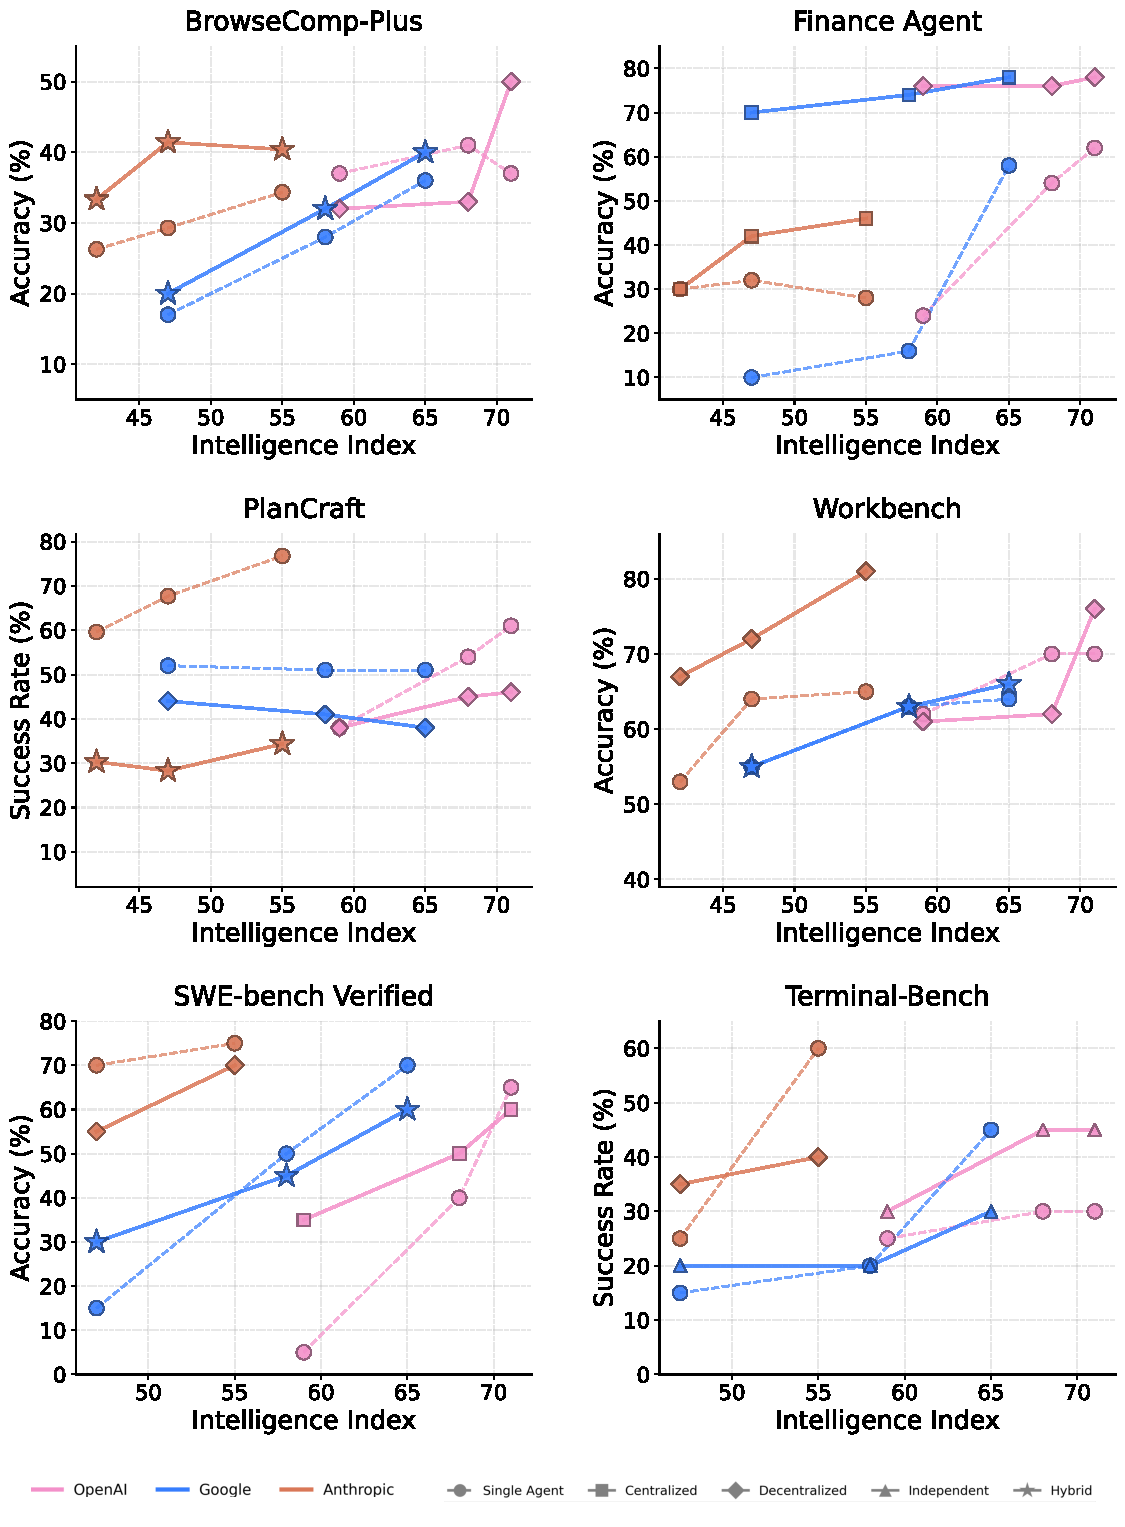
\includegraphics[width=0.9\linewidth]{imgs/main_exp.pdf}
      \caption{\textcolor{black}{\textbf{Agent scaling dynamics across model capability.}
  Performance across six benchmarks show best-performing multi-agent system versus single-agent baselines by Intelligence Index. OpenAI and Google show cooperative scaling in structured tasks (Finance Agent, Workbench). Anthropic models show diminished or negative returns in open-ended environments (PlanCraft, BrowseComp-Plus). SWE-bench Verified and Terminal-Bench show patterns consistent with the capability-saturation threshold: SWE-bench (high SAS baselines) shows limited MAS gains, while Terminal-Bench (lower baselines) shows mixed results with low tool count limiting coordination benefits.}}
      \label{fig:main_exp}
  \end{figure}

% \textcolor{black}{
\section{SWE-bench Verified and Terminal-Bench Results}

\begin{table}[h]
\centering
\small
\caption{Heterogeneous vs. homogeneous agent configurations on BrowseComp-Plus. Centralized heterogeneous configurations uniformly underperform the stronger model's homogeneous baseline; decentralized configurations show modest gains largely attributable to the stronger constituent model.}
\begin{tabular}{llcc}
\toprule
\textbf{Architecture} & \textbf{Configuration} & \textbf{Accuracy} & \textbf{$\Delta$ vs. Homo (strong)} \\
\midrule
Centralized & GPT-5 orch + GPT-5-nano sub & 0.19 & $-$0.15 \\
Centralized & GPT-5-nano orch + GPT-5 sub & 0.21 & $-$0.13 \\
Centralized & Sonnet-4.5 orch + Sonnet-3.7 sub & 0.37 & $-$0.06 \\
Centralized & Sonnet-3.7 orch + Sonnet-4.5 sub & 0.42 & $-$0.01 \\
Centralized & Gemini-2.5-Pro orch + 2.0-Flash sub & 0.18 & $-$0.19 \\
Centralized & Gemini-2.0-Flash orch + 2.5-Pro sub & 0.23 & $-$0.14 \\
Centralized & Gemini-2.5-Pro orch + GPT-5 sub & 0.17 & $-$0.20 \\
\midrule
Decentralized & 2 GPT-5 + 1 GPT-5-nano & 0.56 & $+$0.06 \\
Decentralized & 1 GPT-5 + 2 GPT-5-nano & 0.51 & $+$0.01 \\
Decentralized & 2 Sonnet-4.5 + 1 Sonnet-3.7 & 0.45 & $+$0.02 \\
Decentralized & 1 Sonnet-4.5 + 2 Sonnet-3.7 & 0.48 & $+$0.05 \\
Decentralized & 2 Gemini-2.5-Pro + 1 2.0-Flash & 0.47 & $+$0.04 \\
Decentralized & 1 Gemini-2.5-Pro + 2 2.0-Flash & 0.37 & $-$0.06 \\
\bottomrule
\end{tabular}
\label{tab:s2_heterogeneous}
\end{table}

\begin{table}[h]
\centering
\small
\caption{Regression fit under alternative capability metrics (6-benchmark model, $N=260$). The Agentic Capability Index (ACI) achieves the best cross-validated fit with zero finding reversals.}
\begin{tabular}{lccc}
\toprule
\textbf{Capability Metric} & $R^2_{\text{train}}$ & $R^2_{\text{CV}}$ & \textbf{AIC} \\
\midrule
Intelligence Index & 0.463 & 0.373 & $-$236.3 \\
Agentic Capability Index (ACI) & \textbf{0.481} & \textbf{0.413} & $\mathbf{-244.8}$ \\
Per-dataset SA Baseline & 0.372 & 0.247 & $-$202.0 \\
\bottomrule
\end{tabular}
\label{tab:s3_aci}
\end{table}

\begin{table}[h]
\centering
\small
\caption{Naive vs. cluster-robust $p$-values for key predictors (6-benchmark model, $N=260$, $G=6$ clusters). Predictors varying at the dataset level show substantial SE inflation under cluster-robust inference.}
\begin{tabular}{lccl}
\toprule
\textbf{Predictor} & \textbf{Naive $p$} & \textbf{Robust $p$} & \textbf{Status} \\
\midrule
\texttt{single\_agent\_baseline} & 0.001 & \textbf{0.004} & Survives \\
\texttt{error\_x\_baseline} & 0.022 & \textbf{0.030} & Survives \\
\texttt{log\_tools} & $<$0.001 & 0.172 & Inflated \\
\texttt{intelligence\_centered} & 0.008 & 0.059 & Inflated \\
\texttt{efficiency\_x\_tools} & 0.002 & 0.205 & Inflated \\
\texttt{baseline\_x\_agents} & 0.004 & 0.105 & Inflated \\
\bottomrule
\end{tabular}
\label{tab:s4_cluster}
\end{table}

\begin{table}[h]
\centering
\small
\caption{Holm--Bonferroni multiple comparison correction (19 hypotheses, $\alpha=0.05$). Three predictors survive family-wise error rate correction.}
\begin{tabular}{lccc}
\toprule
\textbf{Predictor} & \textbf{Raw $p$} & \textbf{Holm $p$} & \textbf{Bonferroni $p$} \\
\midrule
\texttt{log\_tools} & $<$0.001 & $<$0.001 & $<$0.001 \\
\texttt{single\_agent\_baseline} & 0.001 & 0.018 & 0.019 \\
\texttt{efficiency\_x\_tools} & 0.002 & 0.026 & 0.030 \\
\midrule
\texttt{intelligence\_centered} & 0.008 & 0.056 & 0.066 \\
\texttt{baseline\_x\_agents} & 0.004 & 0.084 & 0.106 \\
\bottomrule
\end{tabular}
\label{tab:s5_holm}
\end{table}

\begin{table}[h]
\centering
\small
\caption{SWE-bench Verified and Terminal-Bench resolution rates with 95\% bootstrap confidence intervals ($n=20$ instances, 10,000 resamples). Values shown as point estimate [\,lower, upper\,].}
\begin{tabular}{l|ccccc}
\toprule
& \textbf{Single} & \textbf{Centralized} & \textbf{Decentralized} & \textbf{Hybrid} & \textbf{Independent} \\
\midrule
\multicolumn{6}{c}{\textit{SWE-bench Verified}} \\
\midrule
gemini-2.0-flash & 15 [0, 30] & 25 [10, 45] & 25 [5, 45] & 30 [10, 50] & 40 [20, 60] \\
gemini-2.5-flash & 50 [30, 70] & 35 [15, 55] & 35 [15, 55] & 45 [25, 65] & 40 [20, 60] \\
gemini-2.5-pro & 70 [50, 90] & 55 [35, 75] & 45 [25, 65] & 60 [40, 80] & 50 [30, 70] \\
gemini-3-flash & 80 [60, 95] & 75 [55, 95] & 80 [60, 95] & 75 [55, 95] & 60 [40, 80] \\
gpt-5-nano & 5 [0, 15] & 35 [15, 55] & 35 [15, 55] & 30 [10, 50] & 25 [10, 45] \\
gpt-5-mini & 40 [20, 60] & 50 [30, 70] & 30 [10, 50] & 50 [30, 70] & 45 [25, 65] \\
gpt-5 & 65 [45, 85] & 60 [40, 80] & 70 [50, 90] & 55 [35, 75] & 55 [35, 75] \\
claude-sonnet-4 & 70 [50, 90] & 50 [30, 70] & 55 [35, 75] & 45 [25, 65] & 30 [10, 50] \\
claude-sonnet-4-5 & 75 [55, 95] & 70 [50, 90] & 70 [50, 90] & 70 [50, 90] & 55 [35, 75] \\
\midrule
\multicolumn{6}{c}{\textit{Terminal-Bench}} \\
\midrule
gemini-2.0-flash & 15 [0, 30] & 15 [0, 30] & 5 [0, 15] & 5 [0, 15] & 20 [5, 40] \\
gemini-2.5-flash & 20 [5, 40] & 25 [10, 45] & 25 [10, 45] & 25 [10, 45] & 20 [5, 40] \\
gemini-2.5-pro & 45 [25, 65] & 10 [0, 25] & 30 [10, 50] & 25 [10, 45] & 30 [10, 50] \\
gemini-3-flash & 60 [40, 80] & 50 [30, 70] & 55 [35, 75] & 45 [25, 65] & 50 [30, 70] \\
gpt-5-nano & 25 [10, 45] & 20 [5, 40] & 25 [10, 45] & 20 [5, 40] & 30 [10, 50] \\
gpt-5-mini & 30 [10, 50] & 15 [0, 30] & 30 [10, 50] & 20 [5, 40] & 45 [25, 65] \\
gpt-5 & 30 [10, 50] & 45 [25, 65] & 45 [25, 65] & 50 [30, 70] & 45 [25, 65] \\
claude-sonnet-4 & 25 [10, 45] & 25 [5, 45] & 35 [15, 55] & 25 [10, 45] & 35 [15, 55] \\
claude-sonnet-4-5 & 60 [40, 80] & 45 [25, 65] & 40 [20, 60] & 50 [30, 70] & 40 [20, 60] \\
\bottomrule
\end{tabular}
\label{tab:s6_bootstrap}
\end{table}
% }